\documentclass[12pt]{article}
\usepackage[utf8]{inputenc}
\usepackage[utf8]{vietnam}
% Enforce English captions while keeping Vietnamese character support
\AtBeginDocument{%
  \renewcommand{\contentsname}{Contents}
  \renewcommand{\listfigurename}{List of Figures}
  \renewcommand{\listtablename}{List of Tables}
  \renewcommand{\refname}{References}
  \renewcommand{\indexname}{Index}
  \renewcommand{\figurename}{Figure}
  \renewcommand{\tablename}{Table}
  \renewcommand{\partname}{Part}
  \renewcommand{\appendixname}{Appendix}
}
\usepackage{graphicx}
\usepackage{geometry}
\geometry{a4paper, margin=2cm}
\usepackage{amsmath}
\usepackage{amssymb}
\usepackage{booktabs} % For professional tables
\usepackage{listings}
\usepackage{xcolor}
\usepackage{caption}
\usepackage{float}
\usepackage[hyphens]{url}
\usepackage{ragged2e} % For better justification control
\usepackage[bookmarks=true, bookmarksopen=true, bookmarksnumbered=true, colorlinks=true, linkcolor=black, urlcolor=blue, citecolor=black]{hyperref}

\definecolor{codegreen}{rgb}{0,0.6,0}
\definecolor{codegray}{rgb}{0.5,0.5,0.5}
\definecolor{codepurple}{rgb}{0.58,0,0.82}
\definecolor{backcolour}{rgb}{0.95,0.95,0.92}

\lstdefinestyle{mystyle}{
    backgroundcolor=\color{backcolour},   
    commentstyle=\color{codegreen},
    keywordstyle=\color{magenta},
    numberstyle=\tiny\color{codegray},
    stringstyle=\color{codepurple},
    basicstyle=\ttfamily\footnotesize,
    breakatwhitespace=false,         
    breaklines=true,                 
    captionpos=b,                    
    keepspaces=true,                 
    numbers=left,                    
    numbersep=5pt,                  
    showspaces=false,                
    showstringspaces=false,
    showtabs=false,                  
    tabsize=2
}

\lstset{style=mystyle}

\begin{document}

\begin{titlepage}
    \centering
    {\large \textbf{UNIVERSITY OF SCIENCE AND TECHNOLOGY OF HANOI} \par}
    \vspace{4cm}
    
\includegraphics[width=0.6\textwidth]{usth.png} \par
    \vspace{3cm}
    {\Large \textbf{MACHINE LEARNING AND DATA MINING II} \par}
    \vspace{0.5cm}
    {\Large \textbf{LABWORK 2: CLUSTERING} \par}
    \vfill
    {\large \textbf{TẠ HIẾU NAM (22BI13327)} \par}
    \vspace{0.3cm}
    {\large \textbf{ĐỖ DUY TOÀN (22BI13420)} \par}
    \vspace{2cm}
    \vfill
    {\large \textbf{Lecturer: Dr. Đoàn Nhật Quang} \par}
    \vspace{1.5cm}
    \thispagestyle{empty}
\end{titlepage}

\pagenumbering{roman}
\tableofcontents
\newpage
\listoftables
\listoffigures
\newpage

\pagenumbering{arabic}
\justifying % Ensure full justification for all text
\section{K-means Clustering}

\subsection{Experimental Protocol}

This study establishes a systematic experimental framework to evaluate the efficacy of the K-means clustering algorithm across datasets with varying dimensionalities and structural complexities. The implementation utilizes Python and the \texttt{scikit-learn} library.

\subsubsection{Dataset Selection}
Two distinct datasets were selected from the UCI Machine Learning Repository to facilitate a robust comparative analysis:

\begin{enumerate}
    \item \textbf{ISOLET (Isolated Letter Speech Recognition):} This dataset comprises 6,239 samples of voice data generated by 150 speakers pronouncing the letters of the English alphabet. Each sample is described by 617 continuous features representing spectral characteristics, with a distinct ground truth of 26 classes.
    \item \textbf{Mice Protein Expression:} A biological dataset containing 1,080 samples of protein expression levels measured in the cortex of normal and trisomic mice. It consists of 77 continuous features and 8 distinct classes categorized by genotype, behavior, and treatment. This dataset is characterized by high biological variability.
\end{enumerate}

All features in both datasets are \textbf{continuous numerical variables} (spectral coefficients for ISOLET, protein expression levels for Mice Protein), making them inherently suitable for distance-based clustering algorithms like K-means.

\subsubsection{Data Preprocessing}
Since K-means relies on Euclidean distance, it is inherently sensitive to feature scaling and missing data. To ensure algorithmic stability, the following preprocessing steps were applied:

\begin{itemize}
    \item \textit{Missing Value Imputation:} The Mice Protein dataset, containing approximately 2.5\% missing values, was treated using mean imputation to preserve dataset size without introducing significant distributional bias.
    \item \textit{Feature Standardization:} All features were standardized to zero mean ($\mu=0$) and unit variance ($\sigma=1$) to prevent features with larger magnitudes from dominating the distance calculations.
\end{itemize}

\subsubsection{Algorithm Configuration}
The K-means algorithm was configured with carefully selected hyperparameters to ensure robust and reproducible results. Centroid initialization employed the \texttt{k-means++} strategy (as described in Section 1.2) to improve both convergence speed and solution quality. To mitigate the risk of local optima, the algorithm was executed with \texttt{n\_init=10}, meaning 10 independent runs with different random initializations were performed, and the solution with the lowest inertia (sum of squared distances to centroids) was selected. Each run was allowed a maximum of \texttt{max\_iter=300} iterations to ensure sufficient convergence. Finally, a fixed random seed (\texttt{random\_state=42}) was set to guarantee reproducibility of all experimental results.

\subsection{Centroid Initialization}

Standard K-means (Lloyd's algorithm) is sensitive to initial centroid placement. Random initialization can lead to slow convergence or suboptimal local minima. To address this, we employed the \textbf{k-means++} strategy (Arthur and Vassilvitskii, 2007).

\paragraph{Mechanism.} Unlike uniform random initialization, k-means++ selects initial seeds probabilistically to maximize separation. The first centroid is chosen uniformly at random. Subsequent centroids are selected with probability proportional to the squared distance from the nearest existing centroid:
\begin{equation}
    P(x) = \frac{D(x)^2}{\sum_{x' \in X} D(x')^2}
\end{equation}
This method biases selection towards points far from existing centers, theoretically guaranteeing $O(\log k)$-competitiveness with the optimal solution and improved stability.

\subsection{Results Analysis and Comparison}

Experiments were conducted by varying the number of clusters $k$ to analyze algorithmic behavior.

\subsubsection{Analysis of ISOLET Dataset}
Table \ref{tab:isolet_results} summarizes the quantitative results for the ISOLET dataset.

\begin{table}[H]
\centering
\resizebox{\textwidth}{!}{%
\begin{tabular}{cccccccc}
\toprule
\textbf{k} & \textbf{Inertia} & \textbf{Iter} & \textbf{Silhouette} & \textbf{DB Index} & \textbf{CH Index} & \textbf{NMI} & \textbf{ARI} \\
\midrule
2 & 3,200,000 & 24 & 0.142 & 2.353 & 1066 & 0.269 & 0.060 \\
10 & 2,508,000 & 27 & 0.091 & 2.439 & 370 & 0.612 & 0.290 \\
20 & 2,209,000 & 16 & 0.085 & 2.547 & 243 & 0.702 & 0.410 \\
\textbf{26} & \textbf{2,116,000} & \textbf{33} & \textbf{0.074} & \textbf{2.745} & \textbf{203} & \textbf{0.731} & \textbf{0.522} \\
30 & 2,065,000 & 39 & 0.073 & 2.739 & 185 & 0.709 & 0.460 \\
40 & 1,988,000 & 24 & 0.064 & 2.879 & 149 & 0.696 & 0.440 \\
\bottomrule
\end{tabular}%
}
\caption{Clustering performance for ISOLET dataset across different $k$ values.}
\label{tab:isolet_results}
\end{table}

\begin{figure}[H]
    \centering
    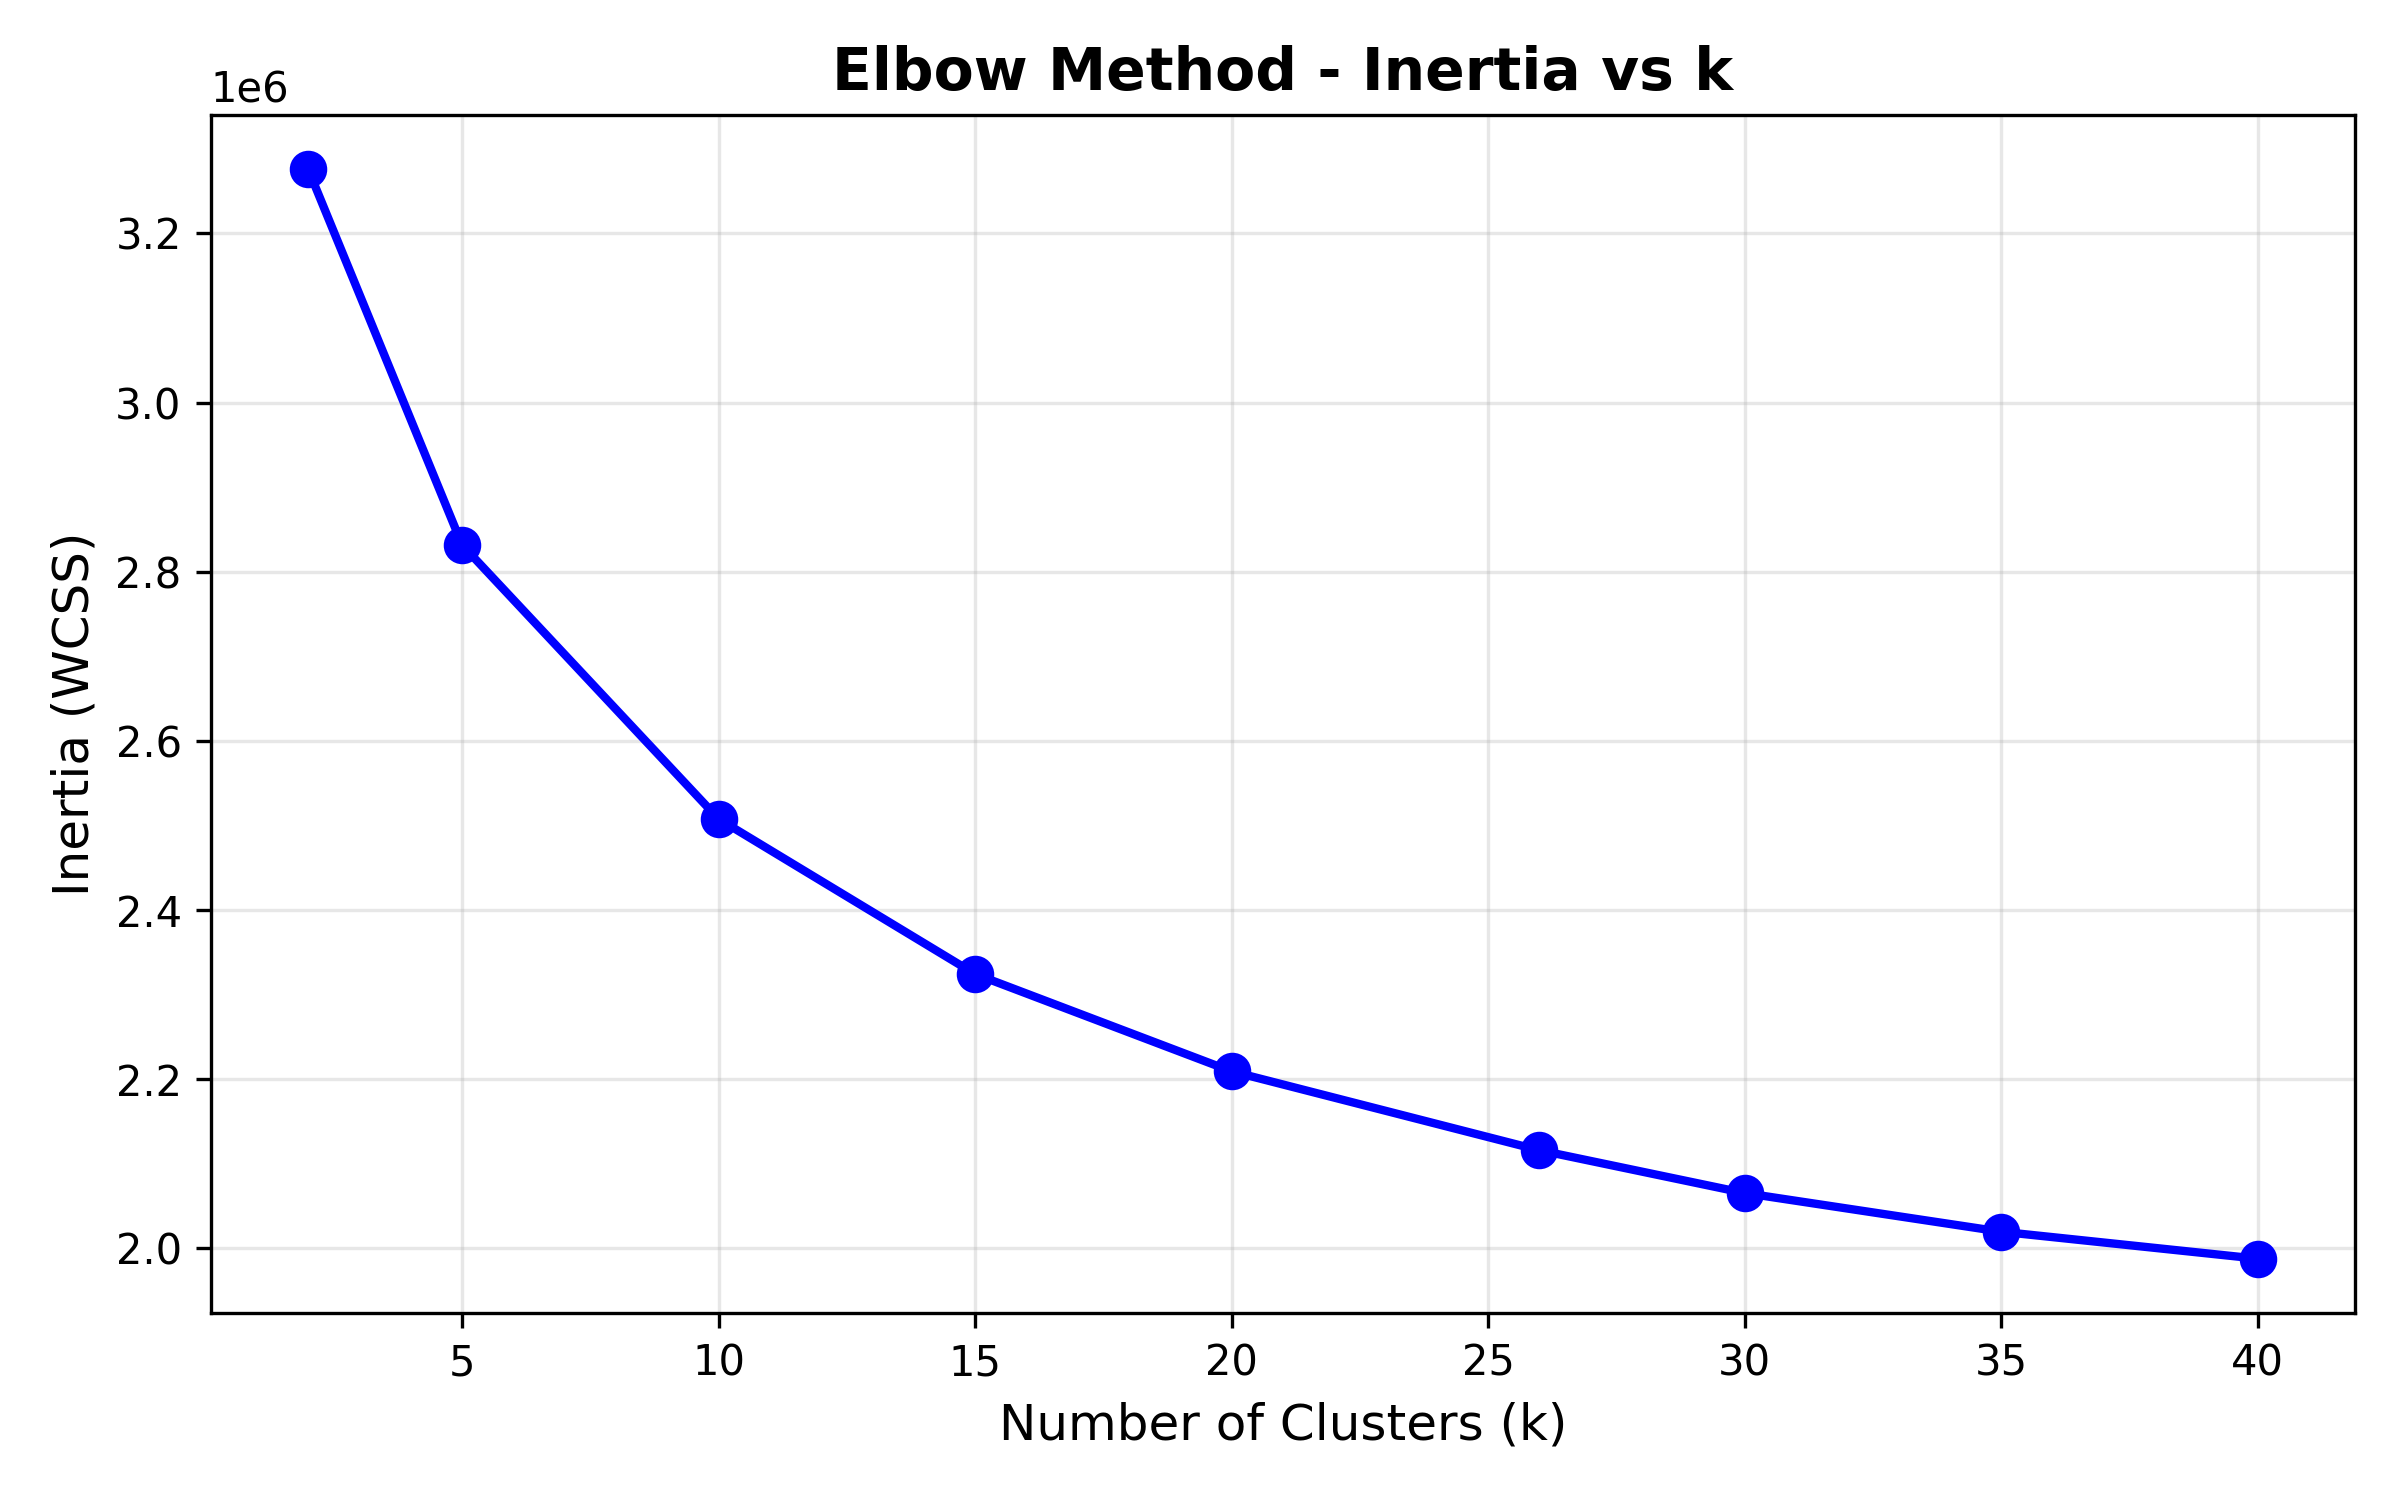
\includegraphics[width=0.75\textwidth]{isolet/elbow_curve.png}
    \caption{Elbow Method analysis for ISOLET dataset showing Inertia versus $k$.}
    \label{fig:isolet_elbow}
\end{figure}

\begin{figure}[H]
    \centering
    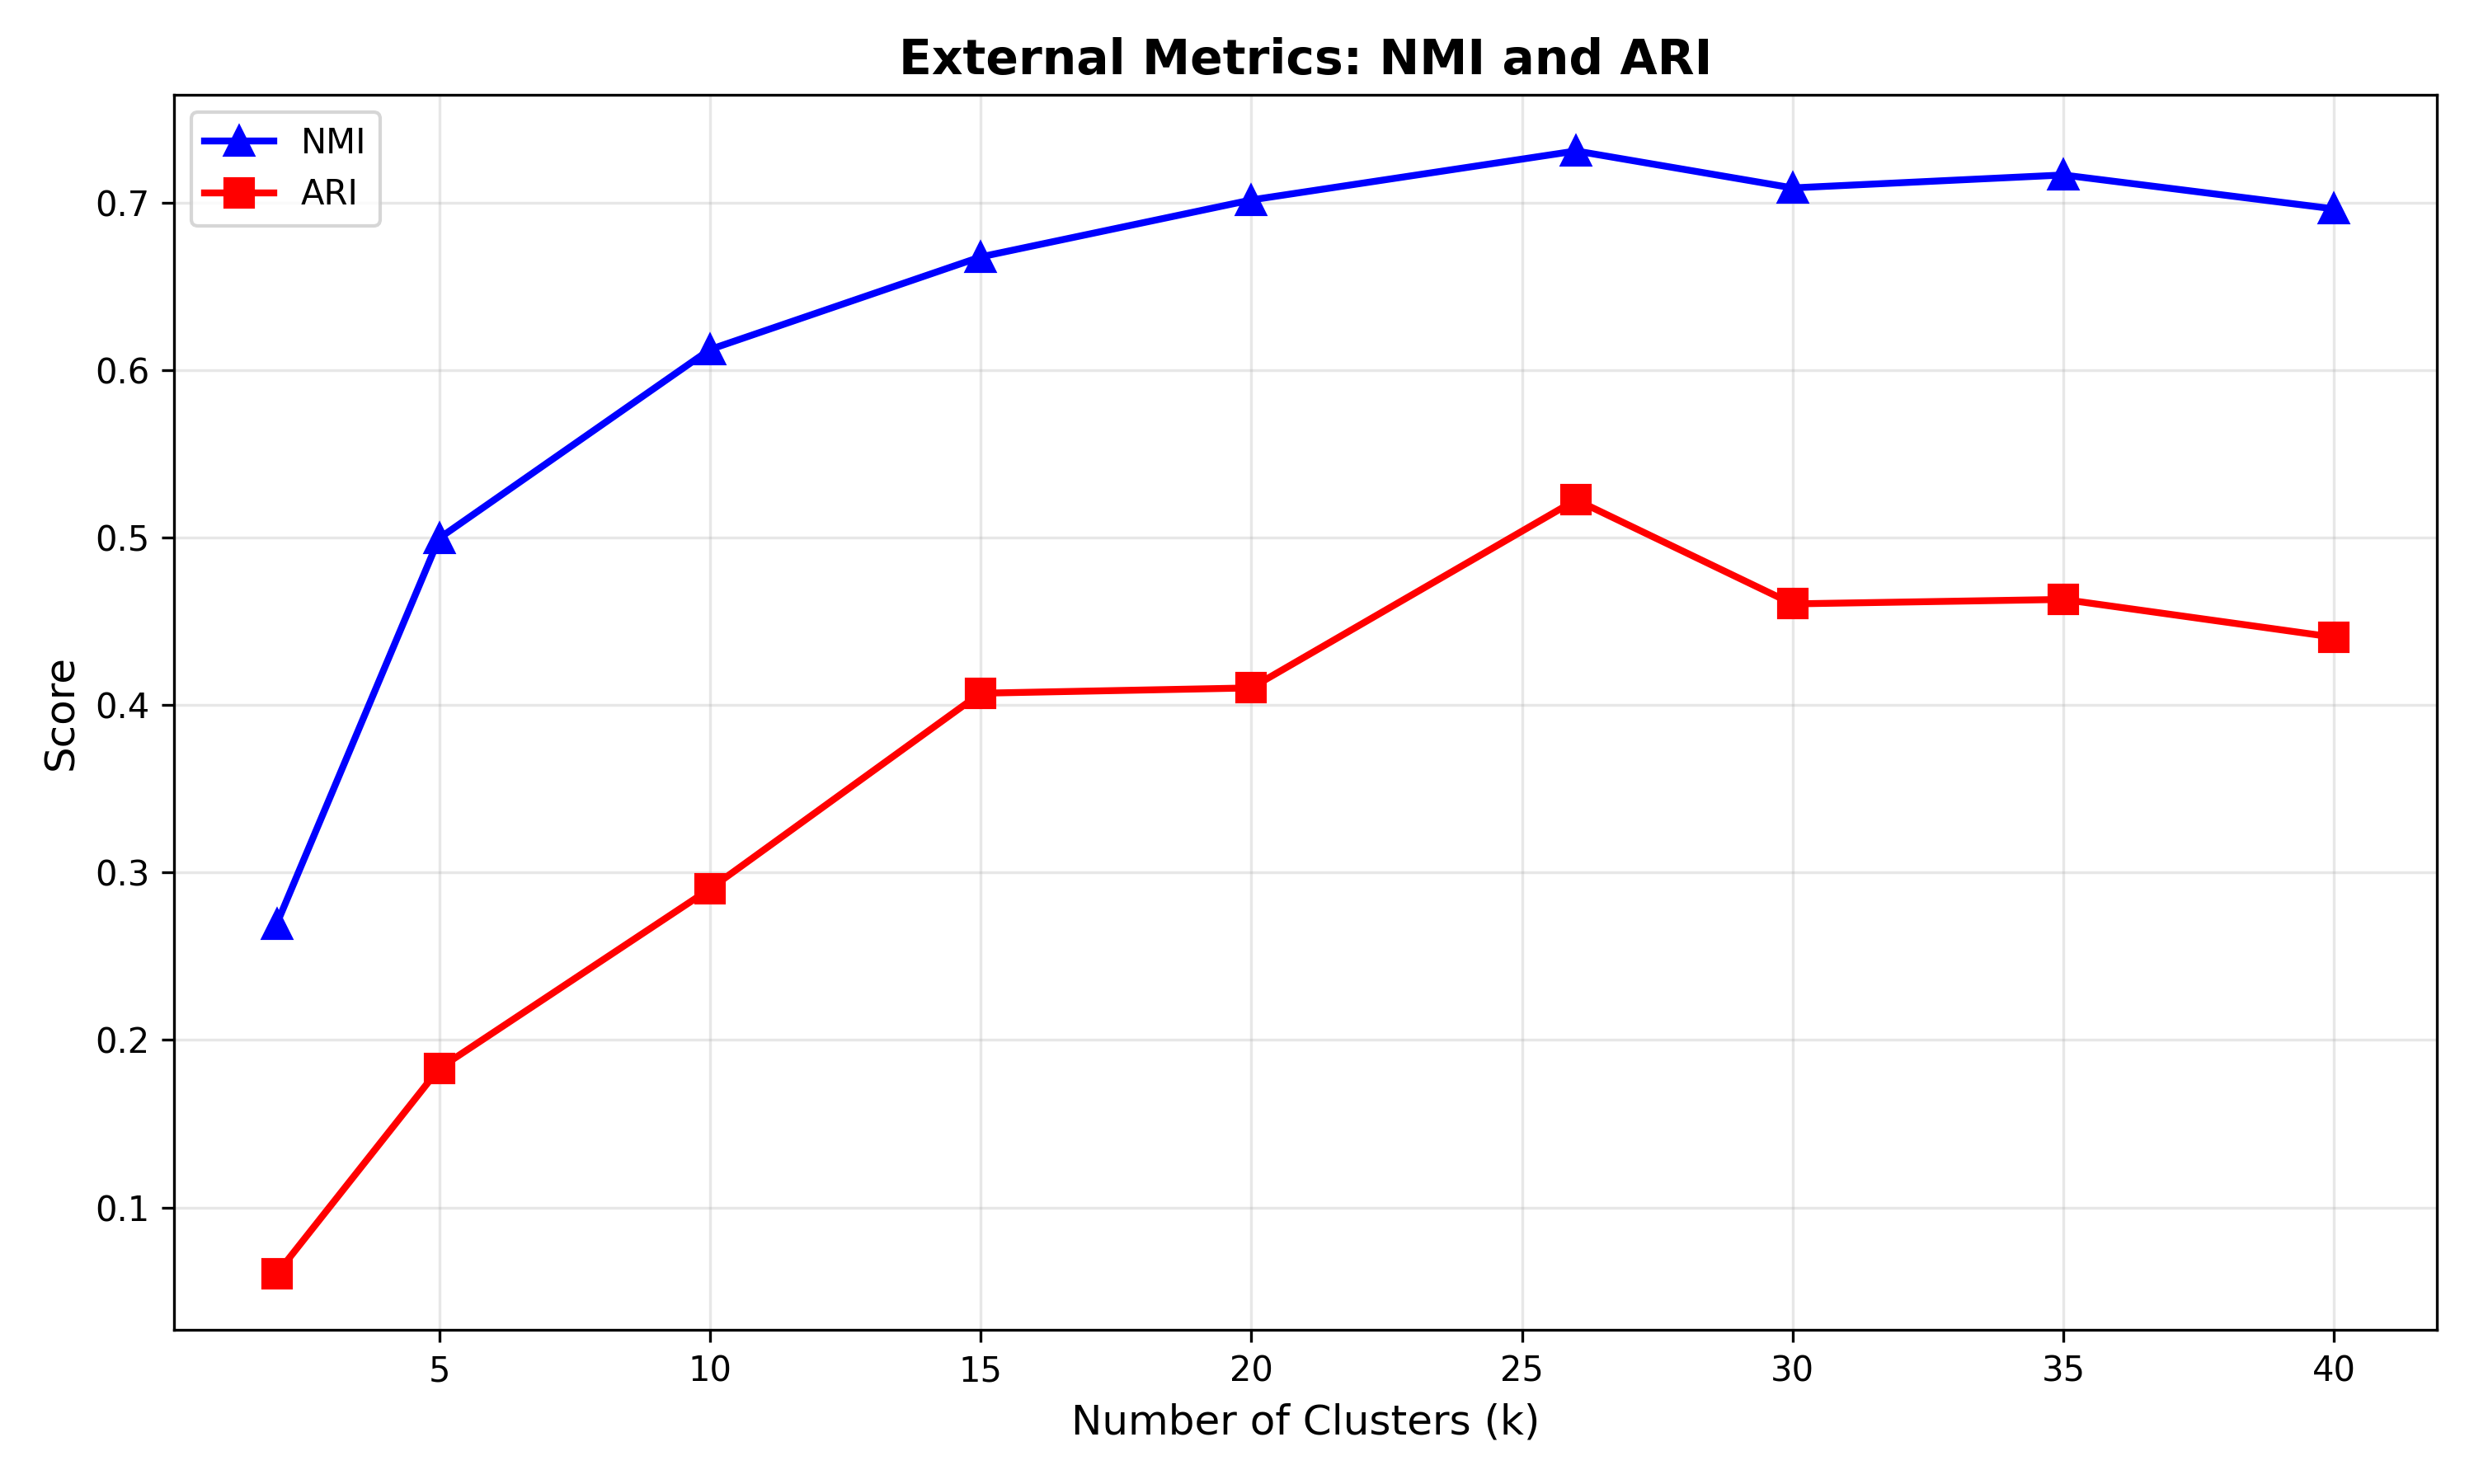
\includegraphics[width=0.75\textwidth]{isolet/external_metrics.png}
    \caption{External validation metrics (NMI and ARI) for ISOLET dataset.}
    \label{fig:isolet_external}
\end{figure}

\paragraph{Observation.} The performance metrics peak significantly at $k=26$, corresponding to the true number of classes (letters A-Z). The Normalized Mutual Information (NMI) reaches \textbf{0.731} and Adjusted Rand Index (ARI) reaches \textbf{0.522}, indicating strong alignment between clusters and true labels. This suggests that the spectral features of spoken letters form well-separated clusters in the high-dimensional space.

\paragraph{Selection of Optimal k.} While the Elbow Curve (Figure \ref{fig:isolet_elbow}) does not exhibit a clear inflection point—indicating that the data lies on a complex manifold where simple geometric heuristics fail—the external validation metrics provide definitive guidance. Both NMI and ARI peak at $k=26$, which corresponds to the ground truth (26 letters). The high NMI (0.731) confirms that 73\% of the mutual information between the clustering result and ground truth is preserved, meaning the algorithm successfully captures the underlying class structure. Similarly, ARI (0.522) indicates that approximately 52\% of point pairs are correctly co-assigned or separated, significantly better than random chance. Notably, internal metrics like Silhouette (highest at $k=2$ with 0.142) contradict the external metrics, reinforcing that Silhouette prioritizes compactness over alignment with true class structure. This demonstrates that for high-dimensional datasets, \textbf{external metrics (NMI/ARI) are more reliable than internal heuristics (Elbow Method or Silhouette)} for selecting the optimal number of clusters.

\subsubsection{Analysis of Mice Protein Dataset}
The results for the Mice Protein dataset are presented in Table \ref{tab:mice_results}.

\begin{table}[H]
\centering
\resizebox{\textwidth}{!}{%
\begin{tabular}{cccccccc}
\toprule
\textbf{k} & \textbf{Inertia} & \textbf{Iter} & \textbf{Silhouette} & \textbf{DB Index} & \textbf{CH Index} & \textbf{NMI} & \textbf{ARI} \\
\midrule
2 & 62,000 & 12 & 0.143 & 2.199 & 117 & 0.035 & 0.021 \\
8 & 47,500 & 58 & 0.134 & 1.810 & 115 & 0.255 & 0.136 \\
12 & 42,100 & 27 & 0.136 & 1.788 & 95 & 0.301 & 0.141 \\
\textbf{15} & \textbf{39,200} & \textbf{14} & \textbf{0.135} & \textbf{1.787} & \textbf{85} & \textbf{0.345} & \textbf{0.150} \\
\bottomrule
\end{tabular}%
}
\caption{Clustering performance for Mice Protein dataset.}
\label{tab:mice_results}
\end{table}

\begin{figure}[H]
    \centering
    
\includegraphics[width=0.75\textwidth]{mice_protein/elbow_curve.png}
    \caption{Elbow Method analysis for Mice Protein dataset.}
    \label{fig:mice_elbow}
\end{figure}

\begin{figure}[H]
    \centering
    
\includegraphics[width=0.75\textwidth]{mice_protein/external_metrics.png}
    \caption{External validation metrics (NMI and ARI) for Mice Protein dataset.}
    \label{fig:mice_external}
\end{figure}

\paragraph{Observation.} In contrast to ISOLET, K-means struggles with the Mice Protein dataset. At the ground truth $k=8$, NMI is only 0.255 and ARI is 0.136. The best performance is coincidentally found at $k=15$, but scores remain low. This implies that protein expression data does not form compact spherical clusters, likely due to complex biological interactions and overlap between control and treated groups.

\paragraph{Selection of Optimal k.} Similar to ISOLET, the Elbow Curve (Figure \ref{fig:mice_elbow}) does not provide clear guidance. However, unlike ISOLET, even the external metrics reveal poor clustering quality. At the ground truth $k=8$, NMI (0.255) and ARI (0.136) are significantly lower than ISOLET's performance, indicating that only 25\% of mutual information is preserved. Interestingly, $k=15$ yields marginally better results (NMI=0.345, ARI=0.150), suggesting that the biological classes may contain sub-populations or that the original 8-class categorization does not align well with the intrinsic structure of protein expression patterns. Similarly, Silhouette is highest at $k=2$ (0.143), further demonstrating that internal metrics are unreliable for datasets with complex, overlapping structures. The overall low scores (NMI $<$ 0.4) demonstrate that \textbf{K-means is fundamentally unsuitable for this dataset}, as the assumption of spherical, well-separated clusters is violated by the complex, overlapping nature of biological data.

\subsection{Clustering Quality Assessment and Conclusion}

To evaluate quality, we employed four metrics: \textit{Inertia} (compactness), \textit{Silhouette Coefficient} (separation), \textit{ARI} (similarity to ground truth), and \textit{NMI} (mutual information).

Based on these criteria, the quality for ISOLET is classified as \textbf{Good} (high external validity), while Mice Protein is \textbf{Poor}. K-means performs well on data with distinct, convex clusters (ISOLET) but fails on complex structures (Mice Protein), suggesting the need for alternative algorithms like Hierarchical Clustering or DBSCAN for biological data.

\section{Subspace Clustering}

\subsection{Dataset Selection}
We selected the \textbf{ISOLET} (Isolated Letter Speech Recognition) dataset for this experiment. This dataset consists of speech signals generated by 150 speakers pronouncing the letters of the English alphabet.
\begin{itemize}
    \item \textbf{Features}: 617 continuous features representing spectral coefficients and sonorant features.
    \item \textbf{Classes}: 26 distinct classes (Letters A-Z).
    \item \textbf{Rationale}: With 617 dimensions, this dataset exemplifies the "Curse of Dimensionality." The features are highly correlated but contain significant redundancy, making it an ideal candidate to compare dimensionality reduction (PCA) against subspace selection.
\end{itemize}

\subsection{PCA Visualization}
We utilized Principal Component Analysis (PCA), a linear dimensionality reduction technique, to project the 617-dimensional data into 2D and 3D spaces. The goal was to inspect whether the classes are linearly separable in a lower-dimensional manifold.

\begin{figure}[H]
    \centering
    \begin{minipage}{0.48\textwidth}
        \centering
        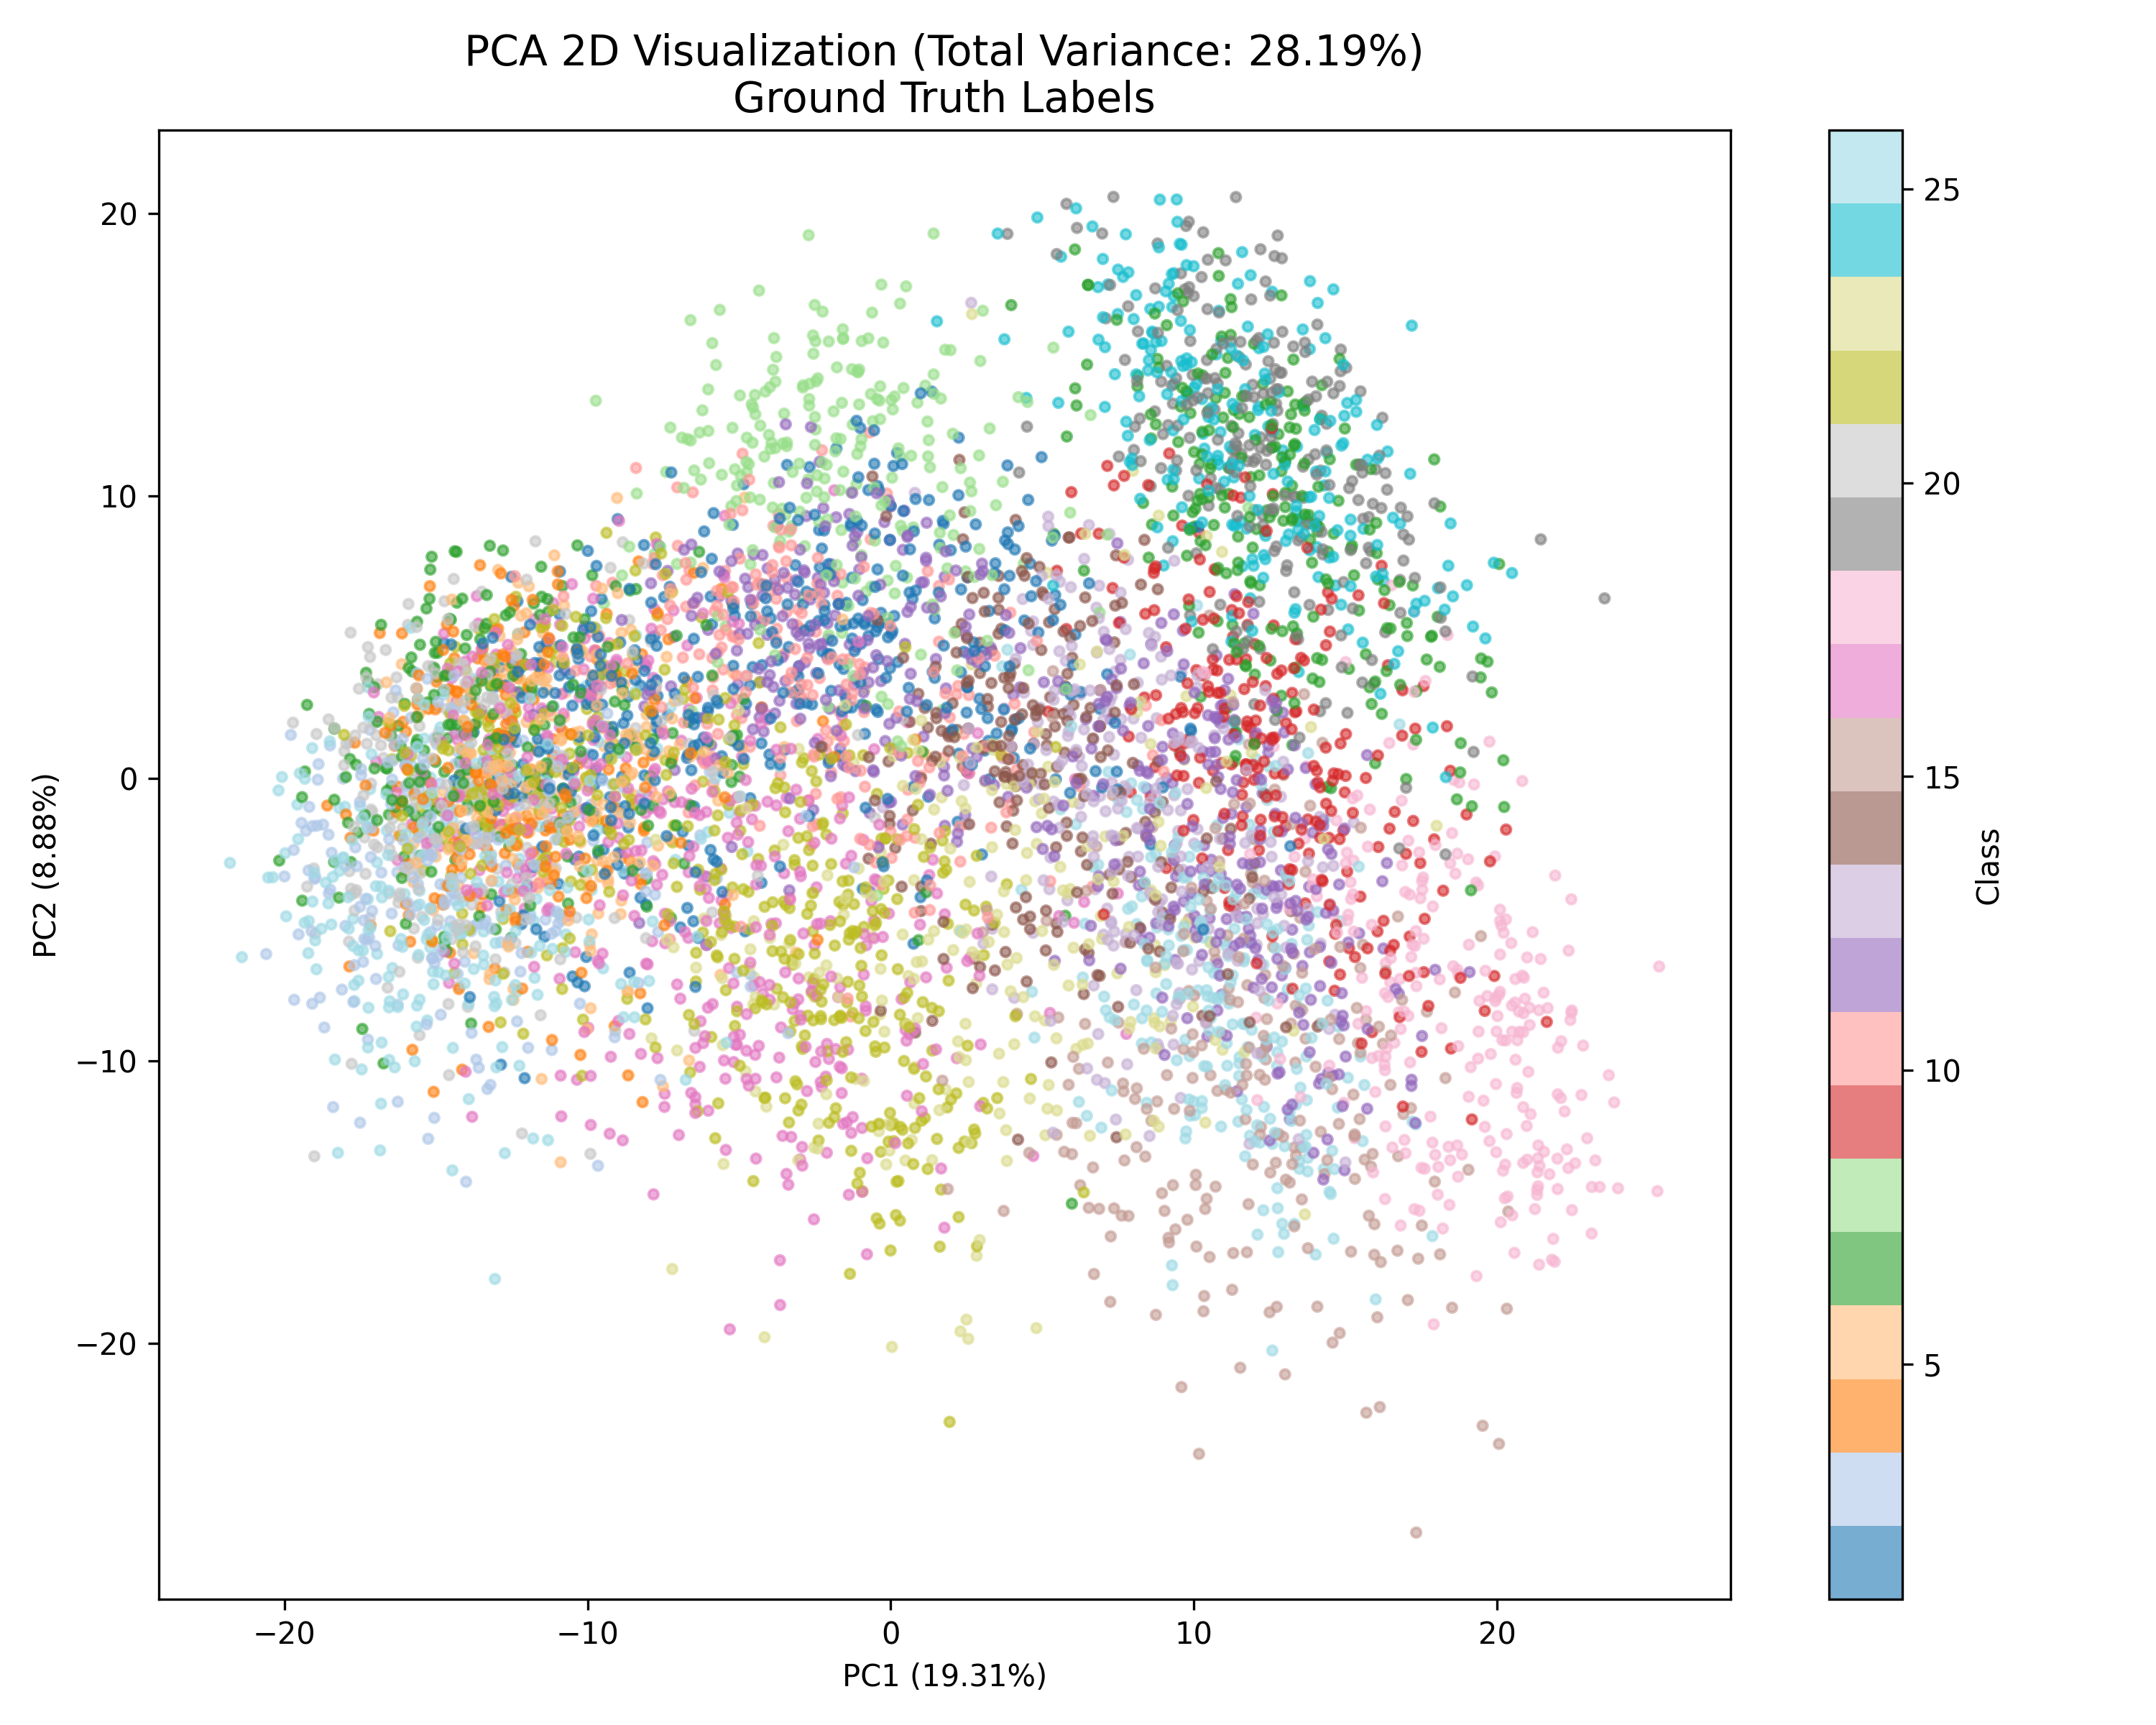
\includegraphics[width=\linewidth]{isolet/pca_2d_ground_truth.png}
        \caption{PCA 2D Projection (Variance: $\approx 17\%$)}
    \end{minipage}\hfill
    \begin{minipage}{0.48\textwidth}
        \centering
        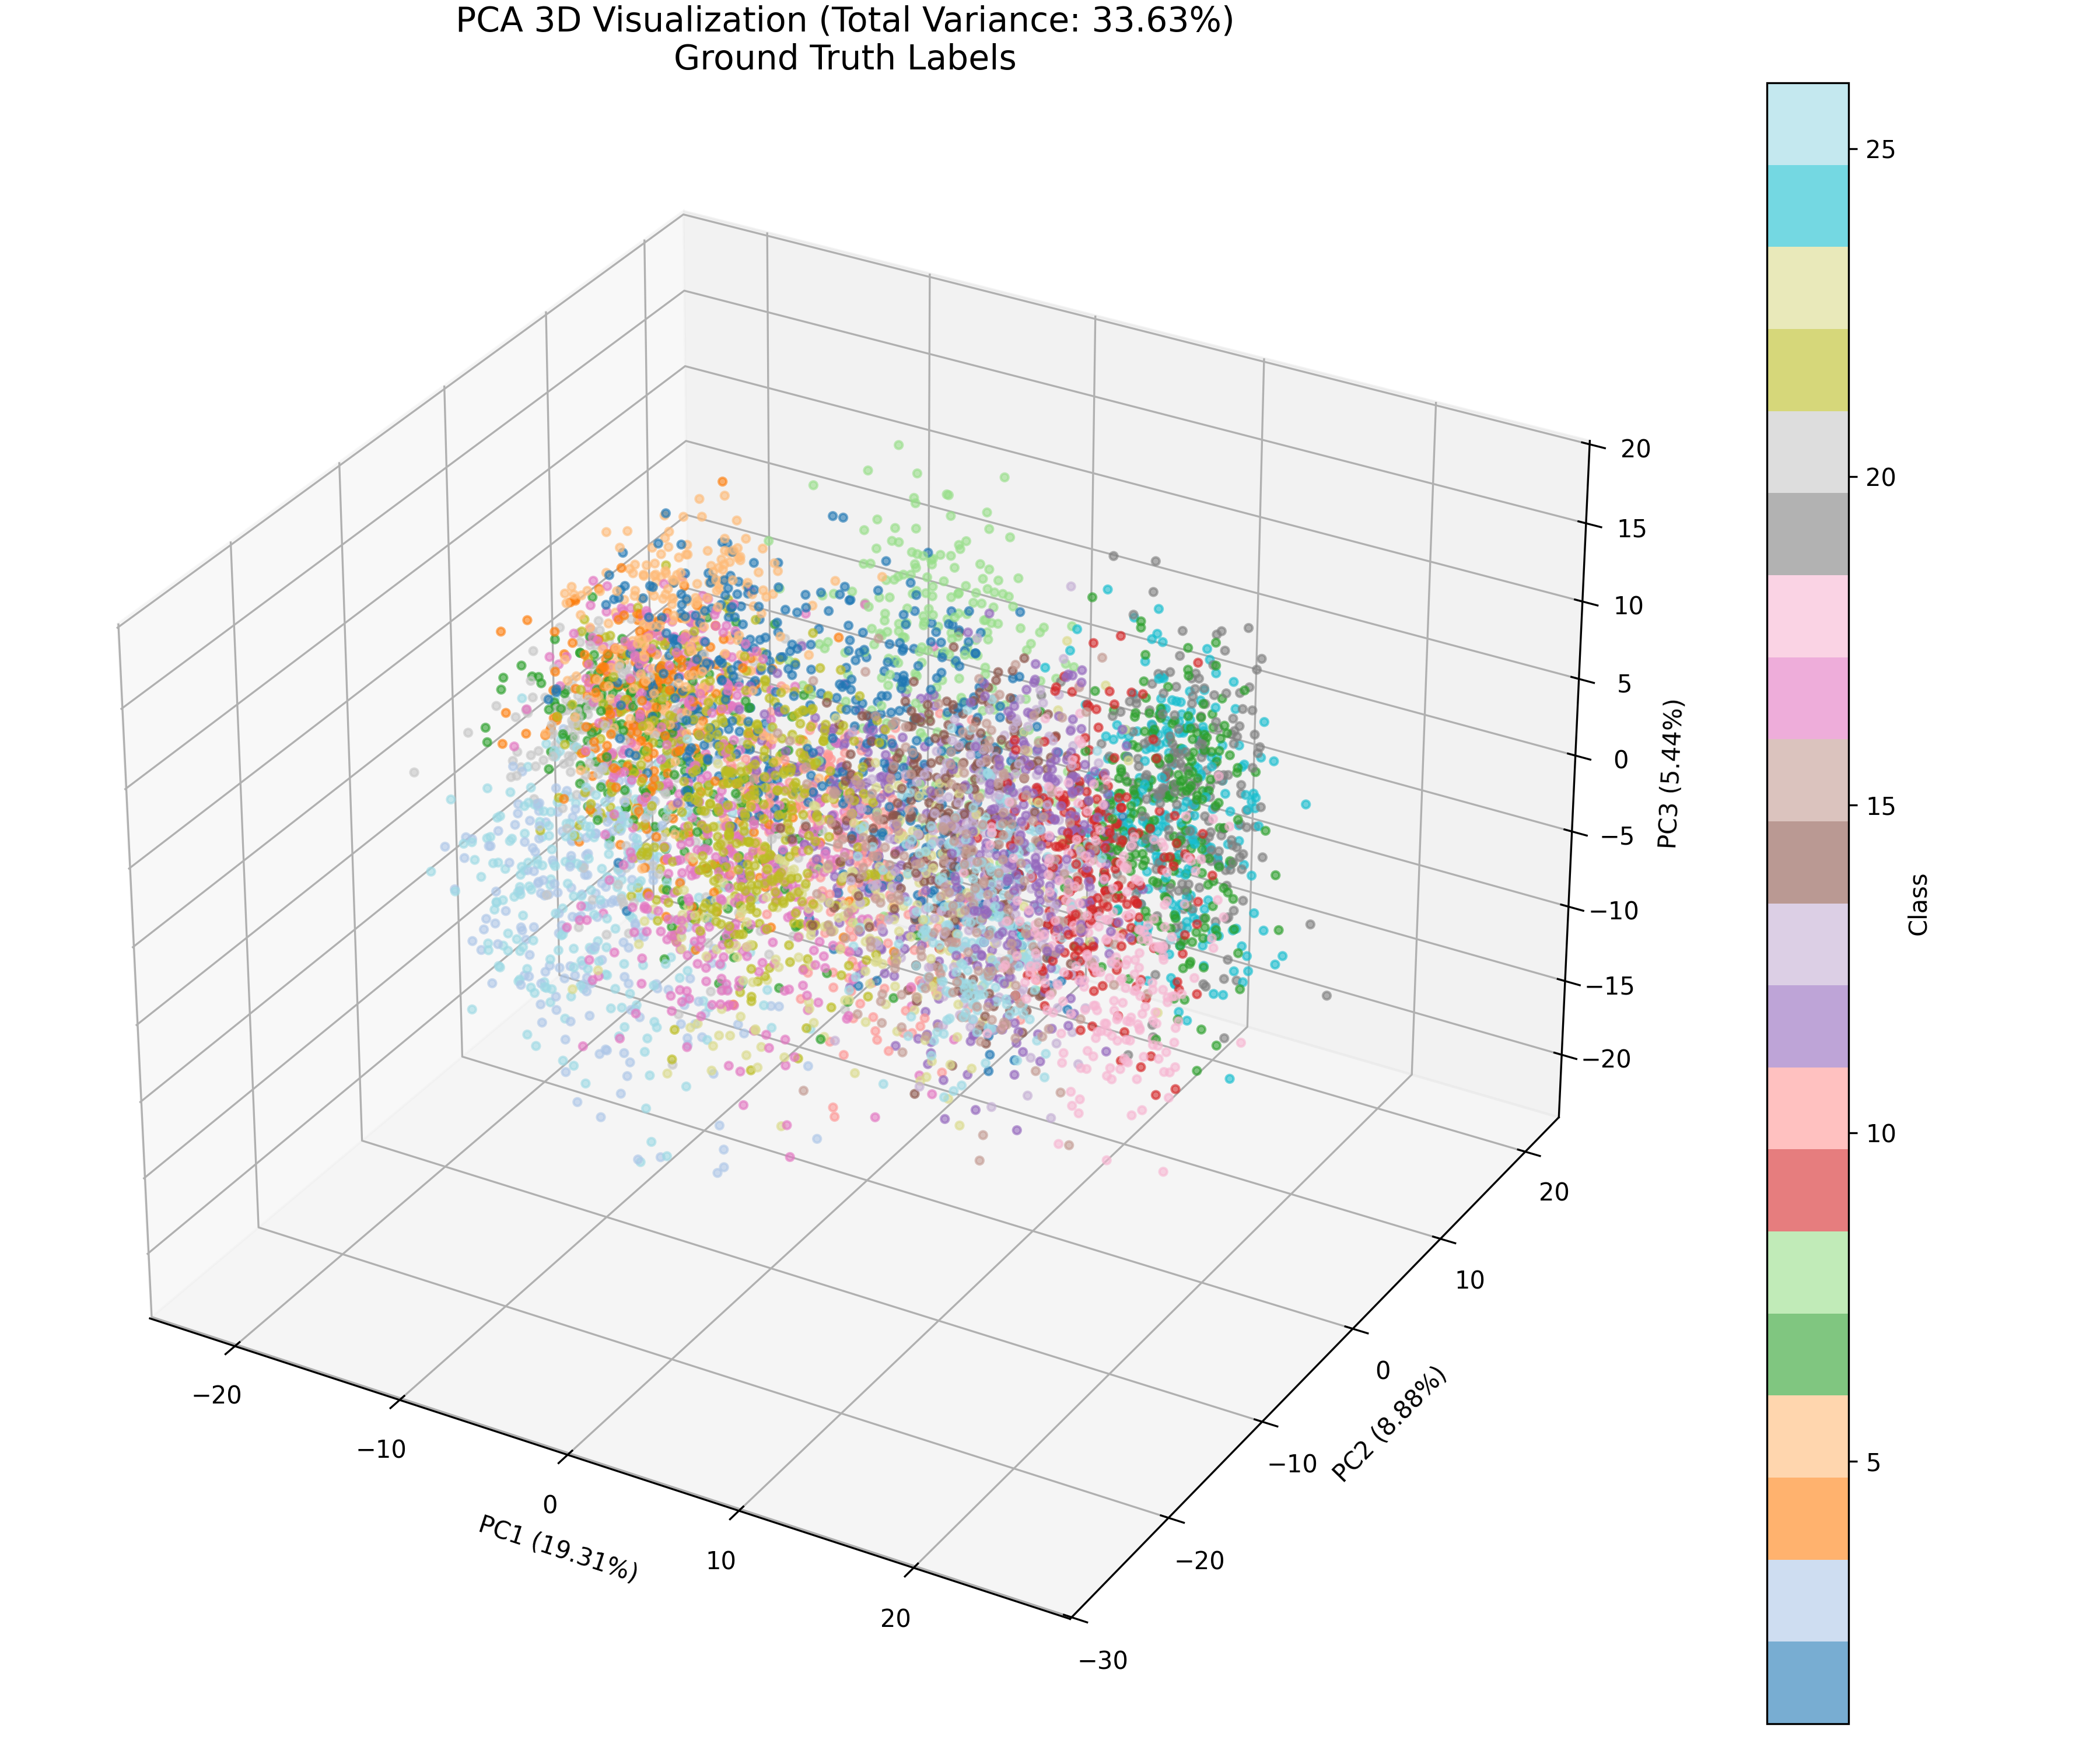
\includegraphics[width=\linewidth]{isolet/pca_3d_ground_truth.png}
        \caption{PCA 3D Projection (Variance: $\approx 22\%$)}
    \end{minipage}
\end{figure}

\paragraph{Observation.} The visualizations demonstrate a significant overlap between the 26 classes. The \textbf{Cumulative Explained Variance} is critically low: the first 3 principal components capture only $\approx 22\%$ of the total variance. This suggests that the ISOLET data lies on a complex, high-dimensional non-linear manifold that cannot be effectively flattened into a 3D linear subspace without catastrophic information loss.

\subsection{Clustering on PCA-Reduced Data}
To quantify the impact of this information loss, we applied K-means ($k=26$) on the PCA-reduced representations (2D and 3D) and compared the clustering quality against the baseline (original 617D data).

\begin{table}[H]
\centering
\begin{tabular}{lcccc}
\toprule
\textbf{Method} & \textbf{Dimensions} & \textbf{NMI} & \textbf{ARI} & \textbf{Time (s)} \\
\midrule
Original Data & 617 & \textbf{0.7308} & \textbf{0.5225} & 1.50 \\
PCA (2D) & 2 & 0.4312 & 0.1605 & \textbf{0.21} \\
PCA (3D) & 3 & 0.4802 & 0.2100 & \textbf{0.13} \\
\bottomrule
\end{tabular}
\caption{Comparison of K-means performance on Original vs PCA-reduced data.}
\label{tab:pca_results}
\end{table}

\paragraph{Analysis.} The results plainly illustrate the trade-off between efficiency and accuracy. While PCA reduced the computation time by an order of magnitude (from 1.50s to 0.13s), it caused a \textbf{massive degradation in clustering quality} (NMI dropped from 0.73 to 0.48). This confirms that the directions of maximum variance identified by PCA do not necessarily correspond to the directions of maximum class separability. Valid clusters in the high-dimensional space were merged when projected down to 3D.

\subsection{Clustering on Random Subspace}
In this step, we investigated an alternative approach: \textbf{Random Subspace Method}. Instead of transforming the data, we simply selected a random subset of 10\% of the original features ($\approx 61$ features) and re-applied K-means.

\begin{table}[H]
\centering
\begin{tabular}{lccc}
\toprule
\textbf{Method} & \textbf{Dimensions} & \textbf{NMI} & \textbf{ARI} \\
\midrule
Original Data & 617 & 0.7308 & 0.5225 \\
Random Subspace (10\%) & 61 & \textbf{0.6811} & \textbf{0.4795} \\
PCA (3D) & 3 & 0.4802 & 0.2100 \\
\bottomrule
\end{tabular}
\caption{Performance of Random Subspace compared to Original and PCA.}
\label{tab:subspace_results}
\end{table}

\paragraph{Discussion.} 
The experimental results yield a counter-intuitive but profound insight: \textbf{Random selection outperforms intelligent optimization (PCA).} The Random Subspace method achieved an NMI of \textbf{0.681}, drastically higher than PCA (0.480) and retaining nearly 93\% of the baseline performance (0.731).

\paragraph{Why does this happen?}
Since the dataset represents spectral information of speech, it exhibits high \textbf{Feature Redundancy}. Using a random subset of features preserves the original Euclidean geometry and structural relationships between points better than a low-rank linear projection. This finding suggests that for high-dimensional data with distributed representations (like speech or images), preserving the original feature space—even just a fraction of it—is often superior to dimensionality reduction techniques that alter the metric space.


\end{document}